\chapter{序論}
\label{chap:introduction}

\section{背景}
\label{section:background}

コンピュータの管理者は,動作中,あるいはカーネルパニックなどによって停止したコンピュータの情報を監視・解析することが必要となる場面がある.
動作中のコンピュータ自身に対しては,同一ホスト内のtopコマンドやpsコマンドを用いて,プロセスの一覧を得たり,gdbコマンドを用いてプロセスをトレースし,プロセスの状態を把握する.
論理的に停止したコンピュータに対しては,kdumpと呼ばれる機構を通してメモリダンプを静的に解析し,原因の究明をする.
また,状態を監視したいホストを物理的なマシンではなく,仮想マシンとして起動し,qemuやXenなどの基盤上でlibvmiなどを通して状態を解析する手法も存在する.

仮想マシン上に起動したホストに対する解析手段としては,上述の通り手段が豊富に揃っている.

これらの課題を解決する手法の一つとして,RDMA NICを用いた解析手法が,(soraさんの論文で)発表された.

\begin{figure}[htbp]
    \caption{libvmiを用いる際のアーキテクチャ}
    \label{fig:zentai}
    \begin{center}
        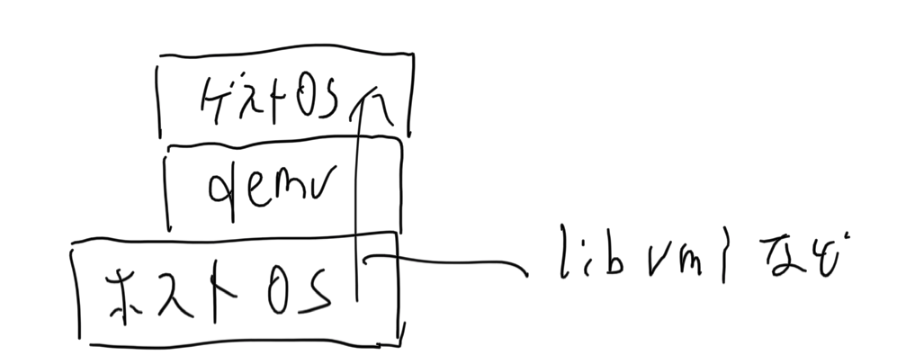
\includegraphics[bb=0 0 1000 340,width=15cm]{img/tegaki/01_vm.png}
    \end{center}
\end{figure}

\section{着目する課題}

% 背景で述べたRDMA NICを用いた解析手法では,メモリの物理アドレスを指定し,逐次的に値を取得し外部から復元していくが,

% これはここに書くべきではない.
% 書くべきは,VMなどの問題点.

Linuxカーネルのバージョン,System.mapの情報およびconfigの情報を知らなければ,メモリのみから正しくコンテキストを復元していくことはできない.

libtlpの論文(もうちょっとちゃんと書く)で紹介されているprocess-list.cはSystem.mapを引数として渡し,
init_taskの行をreadすることでinit_taskの仮想アドレスを得ている.
また,カーネルコンフィグに依存するマクロの値や,使用する関数などもハードコーディングされており,論文の環境以外で動かすことが容易ではない.

\section{目的}
\label{section:purpose}

そこで本研究の目的として,問題の章であげた3つの情報,Linuxカーネルのバージョン,System.mapの情報およびカーネルコンフィグのうち,
System.mapおよびカーネルコンフィグの情報をRDMA NICを用いて復元する.
また,Linuxカーネルのバージョンを知ることさえできれば,どのようなカーネルコンフィグを持つコンピュータに対しても,
RDMA NICを通してプロセスリストの一覧を取得できることを実証する.

この目的を達成するため,本研究では,いくつかの段階に分けてネットワーク越しにあるコンピュータに対して監視・解析を行っていく.
第一の工程として,RDMA NICを用いて,監視対象ホストのメモリを全探索し,
メモリに落ちているSystem.mapのうち,init_taskが配置されている仮想アドレス空間に関する情報と,
Linuxカーネルにおける__phys_addr関数,task_struct型を決定するためのカーネルコンフィグに関する情報を収集する.

次の工程として,収集したカーネルコンフィグを元に手元のコンピュータでLinuxカーネルのソースコードに対してプリプロセスの処理を行い,task_struct型を確定する.
さらに,ソースコード上にある__phys_addrの実体を収集する.

最後に,この工程で得られた情報をもとに,libtlpで提唱されている手法を用いて,プロセスの一覧を正しく取得できることを確認する.

\section{本論文の構成}

こんなことは最後に書く.!!!!!!!!!!!!

\ref{chap:related_works}章では、本研究で使用するlibtlpと,その基盤として使用しているRDMAについて述べる.

\ref{chap:design}章では、RDMAを通してネットワーク越しにあるコンピュータを監視・解析を行うための実行環境の構成に関して述べる.

\ref{chap:implementation}章では、本研究で実装したものについて述べる(加筆)

\ref{chap:evaluation}章では、本研究における評価として,Linuxカーネルのバージョンのみが与えられた状態でプロセスリストの一覧を取得できることを示す.

\ref{chap:conclusion}章では、本研究に関する結論と,今後の課題について述べる.
